\chapter{Implementacija i korisničko sučelje}
		
		
		\section{Korištene tehnologije i alati}
		
			% \textbf{\textit{dio 2. revizije}}
			
			%  \textit{Detaljno navesti sve tehnologije i alate koji su primijenjeni pri izradi dokumentacije i aplikacije. Ukratko ih opisati, te navesti njihovo značenje i mjesto primjene. Za svaki navedeni alat i tehnologiju je potrebno \textbf{navesti internet poveznicu} gdje se mogu preuzeti ili više saznati o njima}.
			
			\subsection{Frontend tehnologije}
            U izradi korisničkog sučelja, točnije \textit{frontend} dijela aplikacije korišten je popularni razvojni okvir \href{https://reactjs.org}{React}. Korištenjem programskog jezika JavaScript React omogućava jednostavnu izradu interaktivnih sučelja temeljenu na React komponentama. Komponente je moguće strukturirati za ponovno korištenje i dijeljenje kroz cijeli projekt (a i druge projekte) što olakšava samu izradu i održavanje. Za uređivanje koda je korišten \href{https://code.visualstudio.com}{Visual Studio Code}.
            \subsection{Backend tehnologije}
			 
		Programski jezik \textit{backend} dijela aplikacije je \href{https://www.java.com/en/download/help/whatis_java.html}{Java}. Korišten je razvojni okvir \href{https://spring.io/projects/spring-boot}{Spring Boot} za čiji je \textit{management} upotrijebljen alat \href{https://maven.apache.org}{Maven}. Tijekom razvoja aplikacije korišten je \href{https://www.h2database.com}{H2} (in-memory) sustav za upravljanje bazama podataka, dok je za \textit{deployanu} verziju korišten sustav \href{https://www.postgresql.org}{PostgreSQL}. Razvojna okruženja korištena na \textit{backendu} su \href{https://www.jetbrains.com/idea/}{InteliJ IDEA} i \href{https://www.eclipse.org}{EclipseIDE}.

            \subsection{Deployment}
            Aplikacija je puštena u pogon na oblaku (engl. cloud) \href{https://render.com}{Render}. Render omogućava povezivanje sa servisom \href{https://gitlab.com}{GitLab} te olakšava puštanje proizvoda u pogon.

            \subsection{Dokumentacija} 
            Za dokumentaciju programskog rješenja korišten je online latex editor. Za crtanje UML dijagrama korišten je Astah i IntelliJ IDEA IDE.

            \subsection{Timska komunikacija} 
            Za timsku komunikaciju korišteni su alati Whatsapp, Discord i Microsoft Teams. 
            
		\section{Ispitivanje programskog rješenja}
			
			%\textbf{\textit{dio 2. revizije}}\\
			 % \textit{U ovom poglavlju je potrebno opisati provedbu ispitivanja implementiranih funkcionalnosti na razini komponenti i na razini cijelog sustava s prikazom odabranih ispitnih slučajeva. Studenti trebaju ispitati temeljnu funkcionalnost i rubne uvjete.}
			\subsection{Ispitivanje komponenti}
			% \textit{Potrebno je provesti ispitivanje jedinica (engl. unit testing) nad razredima koji implementiraju temeljne funkcionalnosti. Razraditi \textbf{minimalno 6 ispitnih slučajeva} u kojima će se ispitati redovni slučajevi, rubni uvjeti te izazivanje pogreške (engl. exception throwing). Poželjno je stvoriti i ispitni slučaj koji koristi funkcionalnosti koje nisu implementirane. Potrebno je priložiti izvorni kôd svih ispitnih slučajeva te prikaz rezultata izvođenja ispita u razvojnom okruženju (prolaz/pad ispita). }
             \noindent \textbf{ 1. ispitni slučaj - pokušaj dodjele rezervacije za trening koji ne postoji}
            \newline U ovom testu ispituje se mogućnost dodjele nepostojeće rezervacije, točnije rezervacije termina treninga koji ne postoji u bazi podataka. Očekuje se iznimka (engl. exception) na servisnom sloju klijenta te ispis poruke u skladu s navedenom iznimkom.
            \begin{figure}[H]
		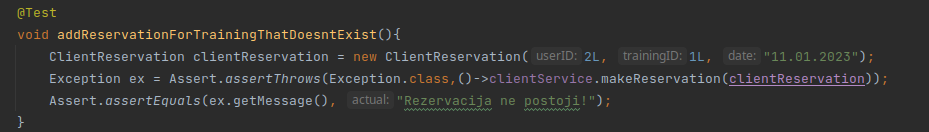
\includegraphics[scale=0.575]{./Slike/test1.png}
		\centering
		\caption{1. test}
		\label{fig:promjene}
	    \end{figure}
            \noindent \textbf{ 2. ispitni slučaj - pokušaj dodjele rezervacije za trening koji nije dodijeljen klijentu}
            \newline U ovom testu ispituje se mogućnost dodjele rezervacije treninga koji nije u treninzima koji su dodijeljeni određenom klijentu, točnije onih koje mu je dodijelio trener. Očekuje se iznimka na servisnom sloju klijenta te ispis poruke u skladu s navedenom iznimkom.
            
            \begin{figure}[H]
		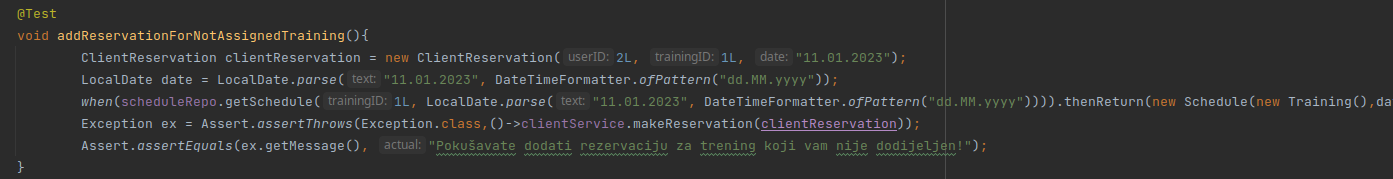
\includegraphics[scale=0.4]{./Slike/test2.png}
		\centering
		\caption{2. test }
		\label{fig:promjene}
	    \end{figure}
            \noindent \textbf{ 3. ispitni slučaj - pokušaj izrade treninga bez prethodne verifikacije od admina}
            \newline U ovom testu ispituje se mogućnost izrade treninga bez prethodne verifikacije trenera od administratora aplikacije. Očekuje se iznimka na servisnom sloju trenera prilikom provjere verfikacije te ispis poruke u skladu s navedenom iznimkom.
            
            \begin{figure}[H]
		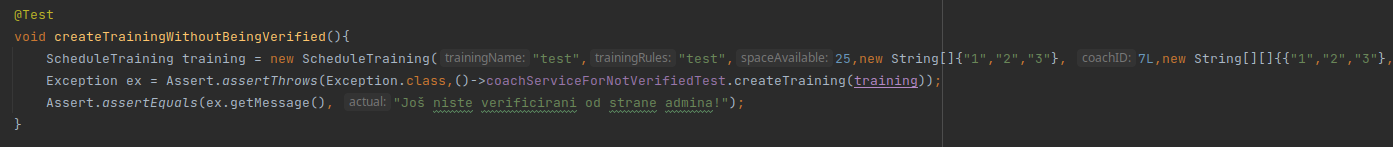
\includegraphics[scale=0.375]{./Slike/test3.png}
		\centering
		\caption{3. test }
		\label{fig:promjene}
	    \end{figure}
            \noindent \textbf{ 4. ispitni slučaj - pokušaj izrade treninga sa prethodnom verifikacijom od admina}
            \newline U ovom testu ispituje se mogućnost izrade treninga nakon verifikacije trenera od administratora aplikacije. Očekuje se uspješna izrada treninga i povratna informacija o istome.
            
            \begin{figure}[H]
		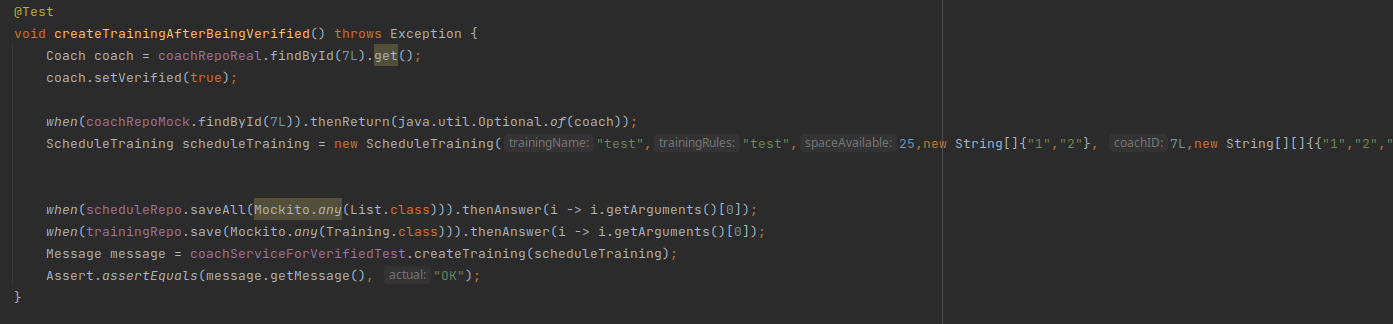
\includegraphics[scale=0.375]{./Slike/test4.png}
		\centering
		\caption{4. test }
		\label{fig:promjene}
	    \end{figure}
            \noindent \textbf{ 5. ispitni slučaj - pokušaja prijave pogrešnom lozinkom}
            \newline U ovom testu ispituje se mogućnost prijave klijenta u aplikaciju pogrešnom lozinkom. Pretpostavka je da je klijent prethodno instanciran i spremljen u bazu podataka s korisničkim imenom kao na slici, a lozinkom password123 te je odgovor servisnog sloja zaduženog za provjeru podataka iznimka s prikladnom porukom o istoj.
     
            \begin{figure}[H]
		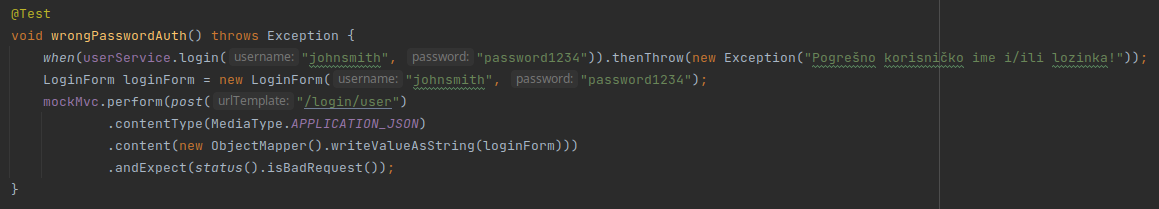
\includegraphics[scale=0.45]{./Slike/test5.png}
		\centering
		\caption{5. test }
		\label{fig:promjene}
	    \end{figure}

            \noindent \textbf{ 6. ispitni slučaj - pokušaj promjene cilja u nepostojeći}
            U ovom testu ispituje se mogućnost promjene cilja klijenta u cilj koji nije definiran unutar baze podataka. Sustav neće dozvoliti takvu promjenu te će se dogoditi iznimka s prikladnom porukom o istoj.
     
            \begin{figure}[H]
		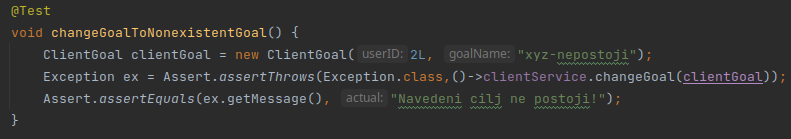
\includegraphics[scale=0.65]{./Slike/test6.png}
		\centering
		\caption{6. test }
		\label{fig:promjene}
	    \end{figure}
     
            \noindent \textbf{Prikaz rezultata testova}
            \newline Testovi komponenti su uspješno provedeni što je vidljivo na priloženoj slici.
            \begin{figure}[H]
		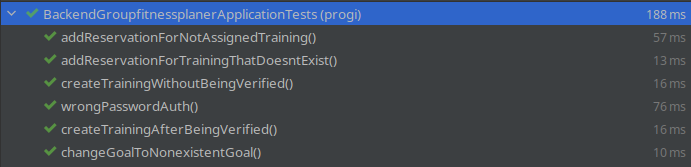
\includegraphics[scale=0.65]{./Slike/test_results.png}
		\centering
		\caption{Rezultati testova }
		\label{fig:promjene}
	    \end{figure}
			
			
			
			\subsection{Ispitivanje sustava}
			
			%  \textit{Potrebno je provesti i opisati ispitivanje sustava koristeći radni okvir Selenium\footnote{\url{https://www.seleniumhq.org/}}. Razraditi \textbf{minimalno 4 ispitna slučaja} u kojima će se ispitati redovni slučajevi, rubni uvjeti te poziv funkcionalnosti koja nije implementirana/izaziva pogrešku kako bi se vidjelo na koji način sustav reagira kada nešto nije u potpunosti ostvareno. Ispitni slučaj se treba sastojati od ulaza (npr. korisničko ime i lozinka), očekivanog izlaza ili rezultata, koraka ispitivanja i dobivenog izlaza ili rezultata.\\ }
			 
			%  \textit{Izradu ispitnih slučajeva pomoću radnog okvira Selenium moguće je provesti pomoću jednog od sljedeća dva alata:}
			%  \begin{itemize}
			%  	\item \textit{dodatak za preglednik \textbf{Selenium IDE} - snimanje korisnikovih akcija radi automatskog ponavljanja ispita	}
			%  	\item \textit{\textbf{Selenium WebDriver} - podrška za pisanje ispita u jezicima Java, C\#, PHP koristeći posebno programsko sučelje.}
			%  \end{itemize}
		 % 	\textit{Detalji o korištenju alata Selenium bit će prikazani na posebnom predavanju tijekom semestra.}
			
			% \eject 

            \noindent \textbf{1. ispitni slučaj sustava: Verifikacija trenera (administrator)}
            \newline \textbf{Postupak}:
            \begin{enumerate}
                
            \item Otvaranje početne stranice

            \item Odabir veze "Pregled korisnika"

            \item Odabir gumba "Potvrdi trenera"

            \item Odabir gumba "OK" u obavještajnom prozoru

            \end{enumerate}
            \textbf{Očekivani rezultati:}
            
		\begin{enumerate}
		    \item Prikaz početne stranice
                \item Prikaz stranice za pregled korisnika
                \item Prikaz obavještajnog prozora s porukom "Jeste li sigurni da želite potvrditi trenera?"
                \item Zatvaranje obavještajnog prozora i uklanjanje gumba "Potvrdi trenera"
		\end{enumerate}
            \begin{figure}[H]
		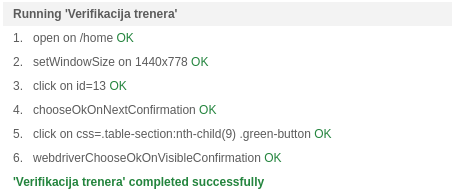
\includegraphics[scale=1]{./Slike/verifikacija_trenera.png}
		\centering
		\caption{1. Selenium test}
		\label{fig:promjene}
	    \end{figure}
     \noindent \textbf{2. ispitni slučaj sustava: Verifikacija trenera (administrator)}
            \newline \textbf{Postupak}:
            \begin{enumerate}
                
            \item Otvaranje početne stranice

            \item Odabir veze "Stvori treninga"

            \item Unos podataka o treningu i terminima treninga

            \item Odabir gumba "Stvori trening"

            \item Odabir gumba "OK" u obavještajnom prozoru

            \end{enumerate}
            \textbf{Očekivani rezultati:}
            
		\begin{enumerate}
		    \item Prikaz početne stranice
                \item Prikaz stranice za izradu treninga
                \item Prikaz obavještajnog prozora s porukom "Uspješno stvoren trening" (nakon 4.)
                \item Zatvaranje obavještajnog prozora
		\end{enumerate}
            \begin{figure}[H]
		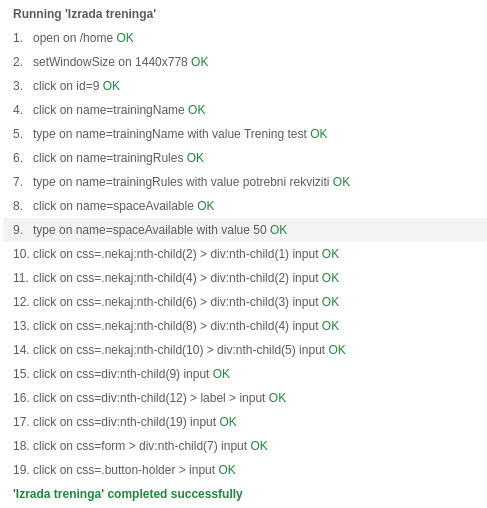
\includegraphics[scale=1]{./Slike/izrada_treninga.png}
		\centering
		\caption{2. Selenium test}
		\label{fig:promjene}
	    \end{figure}
     \noindent \textbf{3. ispitni slučaj sustava: Dodjela treninga klijentu (trener)}
            \newline \textbf{Postupak}:
            \begin{enumerate}
                
            \item Otvaranje početne stranice

            \item Odabir veze "Moji klijenti"

            \item Odabir gumba "Dodijeli trening"

            \item Odabir gumba "Odaberi trening" (moguć višestruki odabir)

            \item Unos fonda sati klijenta

            \item Odabir gumba "Potvrdi odabir"

            \item Odabir gumba "OK" u obavještajnom prozoru

            \end{enumerate}
            \textbf{Očekivani rezultati:}
            
		\begin{enumerate}
		    \item Prikaz početne stranice
                \item Prikaz stranice za pregled klijenata bez treninga
                \item Prikaz stranice za pregled mogućih treninga za dodjelu
                \item Prikaz obavještajnog prozora s porukama "OK" (nakon 6.)
                \item Zatvaranje obavještajnog prozora
		\end{enumerate}
            \begin{figure}[H]
		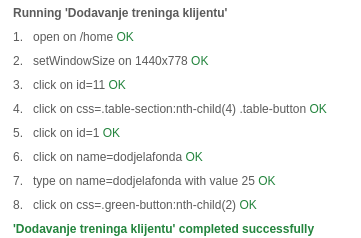
\includegraphics[scale=1]{./Slike/dodjela_treninga_klijentu.png}
		\centering
		\caption{3. Selenium test}
		\label{fig:promjene}
	    \end{figure}
     
     \noindent \textbf{4. ispitni slučaj sustava: Rezervacija termina treninga (klijent)}
            \newline \textbf{Postupak}:
            \begin{enumerate}
                
            \item Otvaranje početne stranice

            \item Odabir veze "Moji treninzi"

            \item Odabir gumba "Odaberi"
            
            \item Odabir gumba "Rezerviraj"

            \item Odabir gumba "OK" u obavještajnom prozoru

            \end{enumerate}
            \textbf{Očekivani rezultati:}
            
		\begin{enumerate}
		    \item Prikaz početne stranice
                \item Prikaz stranice za pregled treninga
                \item Prikaz stranice za pregled termina treninga
                \item Prikaz obavještajnog prozora s porukom "Uspješno ste rezervirali trening!"
                \item Zatvaranje obavještajnog prozora i zatamnjivanje gumba "Rezerviraj"
		\end{enumerate}
            \begin{figure}[H]
		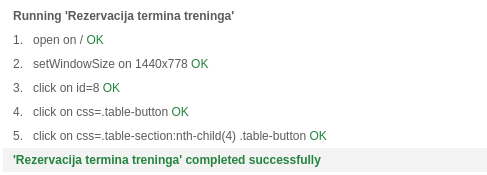
\includegraphics[scale=1]{./Slike/rezervacija_termina_treninga.png}
		\centering
		\caption{4. Selenium test}
		\label{fig:promjene}
	    \end{figure}
		
		\section{Dijagram razmještaja}
			
			% \textbf{\textit{dio 2. revizije}}
			
			 % \textit{Potrebno je umetnuti \textbf{specifikacijski} dijagram razmještaja i opisati ga. Moguće je umjesto specifikacijskog dijagrama razmještaja umetnuti dijagram razmještaja instanci, pod uvjetom da taj dijagram bolje opisuje neki važniji dio sustava.}
                Specifikacijski dijagram razmještaja prikazuje raspodjelu komponenata sustava po lokacijama te odnos sklopovlja i programa. Uočavamo komunikaciju između računala klijenta putem web preglednika i udaljenog poslužitelja (koji sadrži web aplikaciju sa svojim \textit{backend} i \textit{frontend} elementima te poslužitelja baze podataka). Navedena arhitektura sustava naziva se \textit{klijent-poslužitelj} te je u njenoj izvedbi za komunikaciju između dviju navedenih strana korišten protokol HTTP.
			\begin{figure}[H]
		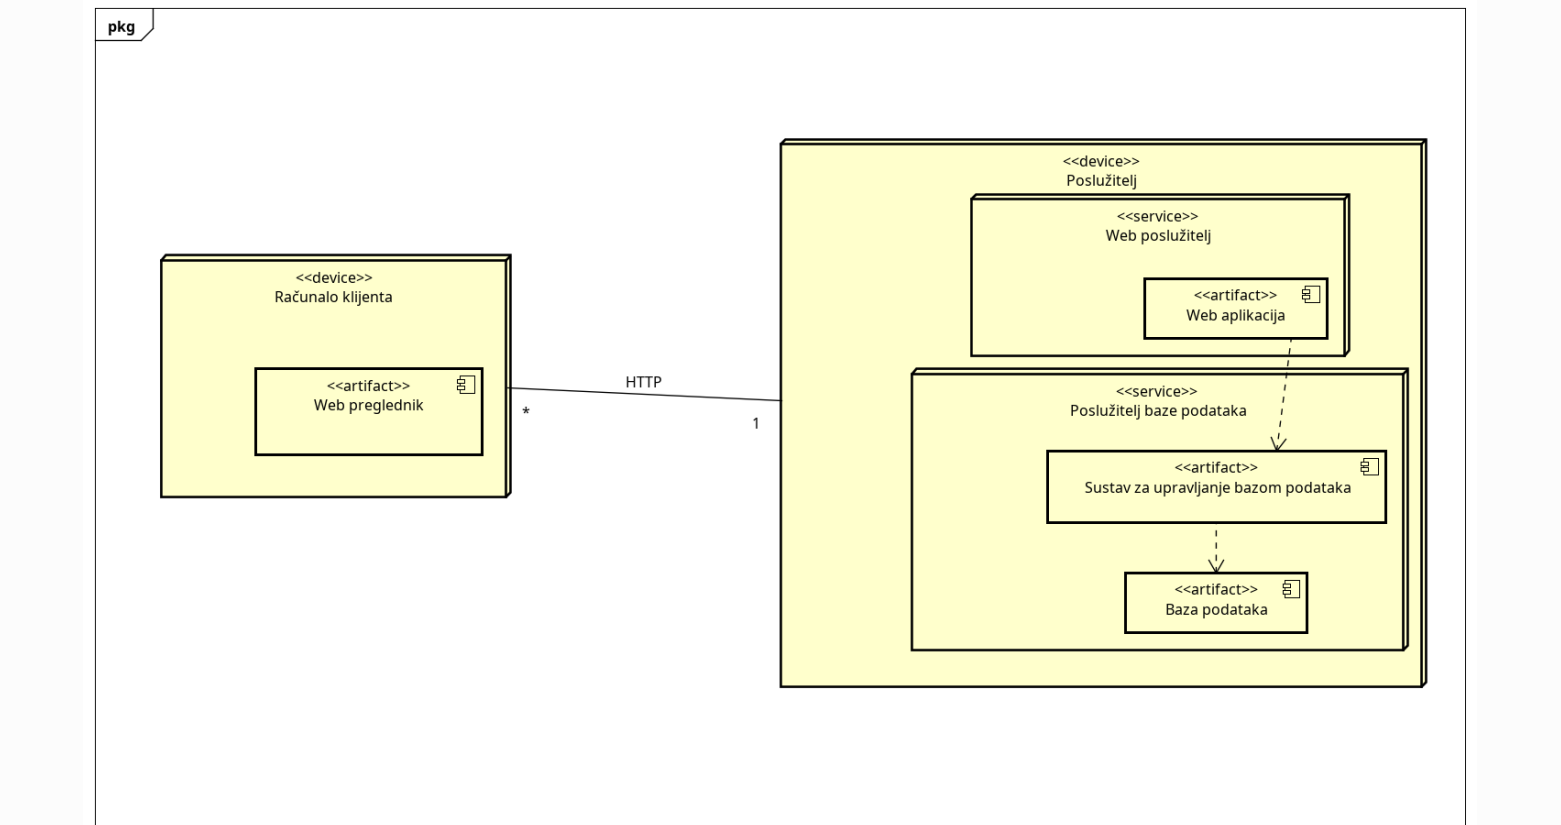
\includegraphics[scale=0.3]{./Dijagrami/dijagram_razmjestaja.png}
		\centering
		\caption{Specifikacijski dijagram razmještaja}
		\label{fig:promjene}
	\end{figure}
			\eject 
		
		
		
		\section{Upute za puštanje u pogon}
            \subsection{Upute za puštanje u pogon na javnom poslužitelju}

            {Aplikacija je puštena u pogon na javnom poslužitelju „Render“. On pruža mogućnost posluživanja web servisa, kao i PostgreSQL baze podataka.\\
            Puštanje u pogon sadržava korake:
            \item \textbf{- kreiranje baze podataka}
            \item \textbf{- puštanje backenda u pogon na javnom poslužitelju}
            \item \textbf{- puštanje frontenda u pogon na javom poslužitelju\\}

            {Bazu podataka kreirali smo i njome upravljamo diretkno iz servisa Render, jer on omogućuje tu opciju. Baza sadržava podatke potrebne za njeno povezivanje sa web servisima. }
            \begin{figure}[H]
                      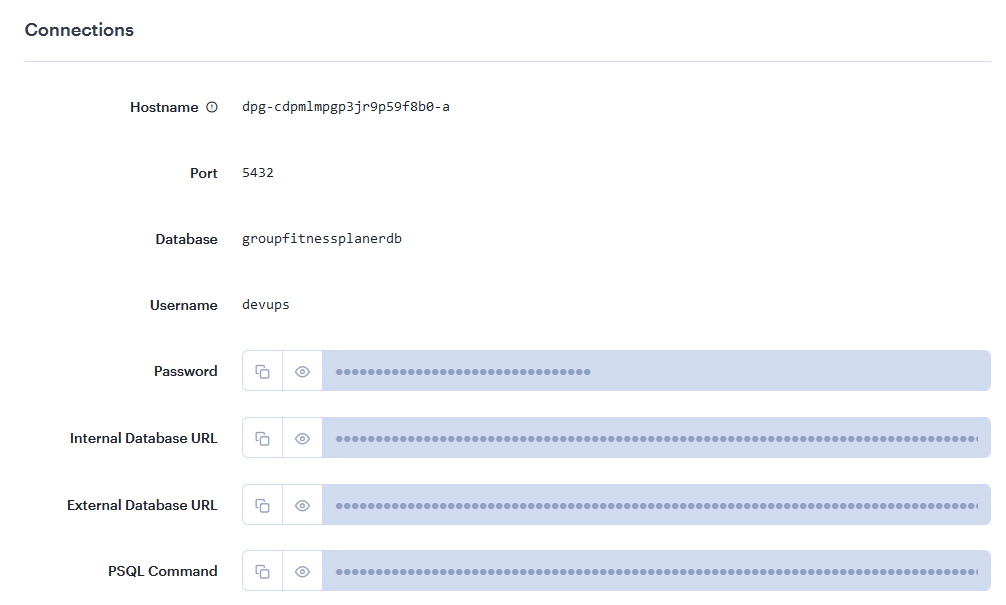
\includegraphics[scale=0.5]{./Slike/baza.png}
                      \centering
                      \caption{Render sučelje za upravljanje bazom podataka}
                      \label{fig:promjene}
                \end{figure}

            {Kako bismo uspješno prenjeli backend aplikacije na web poslužitelj, bilo je potrebno dodati Dockerfile koji upravlja i posreduje komunikaciji backenda i Mavena, alata pomoću kojeg Java projekti postaju sinkronizirani sa Apache HTTP serverima. Također, bilo je potrebno povezati kreiranu bazu podataka sa backendom. Konfiguracija environment varijabli u application.properties datoteci svojstava nužno je da bismo mogli postavili adresu, korisničko ime i lozinku baze podataka na produkciji. Također, opcija kreiranja web servisa u Renderu zahtjeva dodavanje potrebnih varijabli okruženja koje treba kopirati iz danih connections-a baze podataka, postavljanje putanje za Dockerfile. }
            \begin{figure}[H]
                      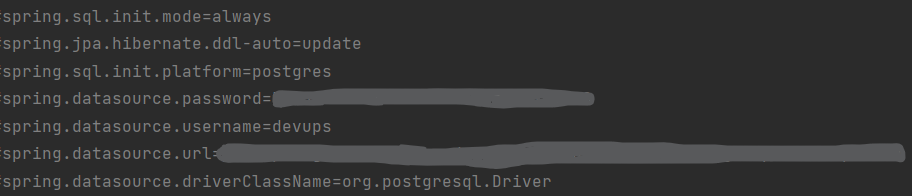
\includegraphics[scale=0.5]{./Slike/config.png}
                      \centering
                      \caption{Konfiguracija postavki za povezivanje backenda sa bazom podataka}
                      \label{fig:promjene}
                \end{figure}

            {Kako bismo uspješno prenjeli frontend, bilo je potrebno u package.json dodati zavisnosti potrebne za puštanje u pogon, primarno proxy-middleware, dotnev, express. Također, bilo je potrebno dodati setupProxy.js koji služi kao server za lokalno razvijanje, app.js u kojem se nalazi express server za produkcijski proxy, kao i izmjeniti package.json dodavanjem "start-prod": "node app.js" skripte, koja navigira front da komunicira preko app.js filea. Opcija kreiranja web servisa u Renderu zahtjevala je postavljanje build komande i start komande, dodavanje variabli okruženja koje pokazuju na adresu backenda koji je prethodno pušten u pogon na javom poslužitelju kako bi javni frontend bio povezan za backendom (koji je povezan sa bazom podataka). \\
            URL na javnu verziju aplikacije: \href{https://group-fitness-planer-q3fc.onrender.com}{https://group-fitness-planer-q3fc.onrender.com}\\}

            \subsection{Upute za puštanje u pogon lokalno\\}
            
            {Aplikaciju također možemo u pogon puštati lokalno, za potrebe razvoja. Taj postupak podijeljen je u dva glavna koraka: 
            \item \textbf{- puštanje backenda lokalno}
            \item \textbf{- puštanje frontenda lokalno\\}}

            {Backend se pokreće iz IDE-a (IntelliJ, Eclipse…) pokretanjem datoteke: GroupFitnessPlannerApplication.java (putanja glasi: /group-fitness-planer/Backend/\\src/main/java/progi/GroupFitnessPlannerApplication.java), koja je autogenerirani dokument svakog Spring boot projekta. Ono što omogućuje lokalno pokretanje su svojstva aplikacije u application.properties koja su postavljena kao na idućoj slici: }
             \begin{figure}[H]
                      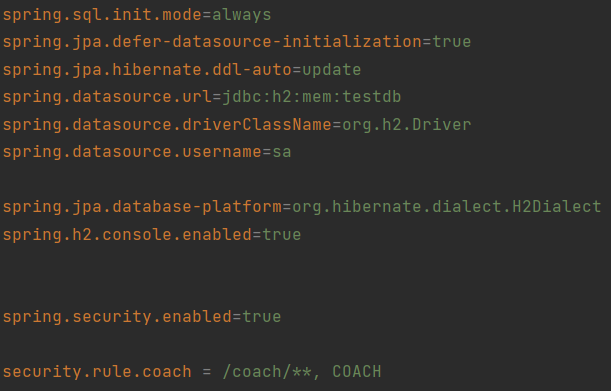
\includegraphics[scale=0.7]{./Slike/lokalno.png}
                      \centering
                      \caption{Konfiguracija postavki za pokretanje backenda lokalno}
                      \label{fig:promjene}
                \end{figure}

            {Za potrebe razvoja koristili smo se in-memory h2 bazom podataka. Aplikacija se pokreće na localhost:8080 portu. Ukoliko želimo prelgedavati stanje u bazi, koristimo URL: localhost:8080/h2-console. }
            \begin{figure}[H]
                      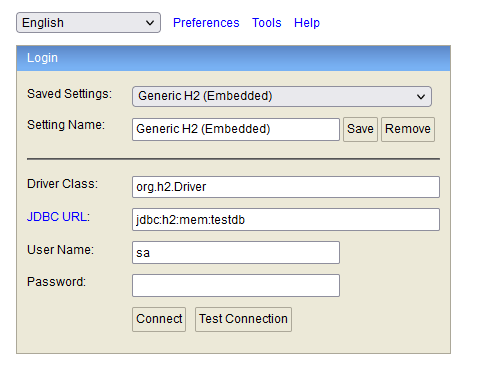
\includegraphics[scale=0.7]{./Slike/h2baza.png}
                      \centering
                      \caption{Konzola za in-memory bazu}
                      \label{fig:promjene}
                \end{figure}

            {Pokretanje frontenda obavlja se iz naredbenog retka. Najprije se pozicioniramo u direktorij sa package.json fileom (/group-fitness-planer/Frontend/groupfitnessui) i u njemu izvedemo naredbe:\\ 
            \textbf{npm install} \\
            koja instalira sve node module potrebne za pokretanje aplikacije, te \\
            \textbf{npm start} \\
            koja pokreće aplikaciju na localhost:8080 (namješteno tako da se front i back pokreću na istom portu kako bi mogli komunicirati). Stranica se ponovno učitava svakom spremljenom promjenom u kodu. 
            \\}
            
}
		
			%\textbf{\textit{dio 2. revizije}}\\
		
			 %\textit{U ovom poglavlju potrebno je dati upute za puštanje u pogon (engl. deployment) ostvarene aplikacije. Na primjer, za web aplikacije, opisati postupak kojim se od izvornog kôda dolazi do potpuno postavljene baze podataka i poslužitelja koji odgovara na upite korisnika. Za mobilnu aplikaciju, postupak kojim se aplikacija izgradi, te postavi na neku od trgovina. Za stolnu (engl. desktop) aplikaciju, postupak kojim se aplikacija instalira na računalo. Ukoliko mobilne i stolne aplikacije komuniciraju s poslužiteljem i/ili bazom podataka, opisati i postupak njihovog postavljanja. Pri izradi uputa preporučuje se \textbf{naglasiti korake instalacije uporabom natuknica} te koristiti što je više moguće \textbf{slike ekrana} (engl. screenshots) kako bi upute bile jasne i jednostavne za slijediti.}
			
			
			 %\textit{Dovršenu aplikaciju potrebno je pokrenuti na javno dostupnom poslužitelju. Studentima se preporuča korištenje neke od sljedećih besplatnih usluga: \href{https://aws.amazon.com/}{Amazon AWS}, \href{https://azure.microsoft.com/en-us/}{Microsoft Azure} ili \href{https://www.heroku.com/}{Heroku}. Mobilne aplikacije trebaju biti objavljene na F-Droid, Google Play ili Amazon App trgovini.}
			
			
			\eject 